\subsection{CFCSS}

Unlike the usual implementation, which works over assembly instructions, or LLVM's \acrfull{ir}, our implementation takes advantage of Rust's macro system to insert \acrshort{cfcss} directly into program code. An algorithm originally designed for LLVM \acrshort{ir} \cite{coast:cfcss} is used, with modifications to make it suitable for our purposes.

Macro is used to designate a \textit{module} as \acrshort{cfcss} protected, each function within the module being designated as a \textit{block} ({$b_n$}). A graph is then generated at compile time representing the allowed control flow within the protected module. Each block within the graph is assigned a random unique signature ({$s_n$}) and signature difference ({$d_n$}), which is calculated by XORing ({$\oplus$}) the current block's signature and the signature of its predecessor as seen in equation \ref{eq:block_diff}.

\begin{equation}
d_n = s_n \oplus s_{n-1}
\label{eq:block_diff}
\end{equation}

\begin{figure}[!h]
    \centering
    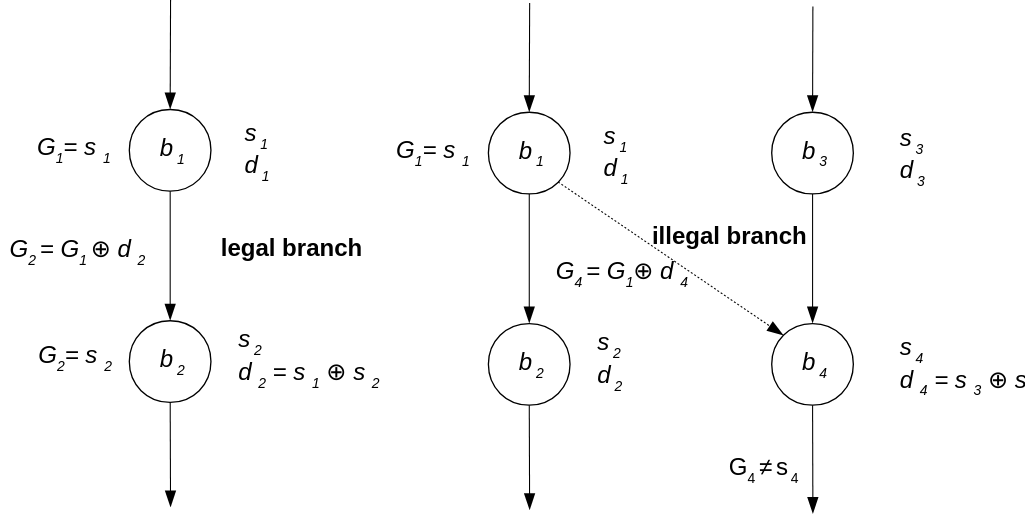
\includegraphics[width=1.0\textwidth]{diagrams/cfcss/basic.png}
    \caption{Basic \acrshort{cfcss} \cite{coast:cfcss}}
\end{figure}

A runtime signature {$G_n$} is also created for the given protected module, initially set to {$G_0 = 0$}. This signature is updated at runtime before the execution of every block by XORing it with the signature difference of the destination block (equation \ref{eq:runtime_sig}). Using XOR to update the runtime signature is favorable, since XOR operation can be undone by simply being repeated, which is desirable when returning from a block.

\begin{equation}
\label{eq:runtime_sig}
G_n = G_{n-1} \oplus d_n
\end{equation}

To ensure correct control flow, the newly calculated runtime signature must be equal to the function signature, otherwise an invalid branching occurred.

\begin{equation}
\label{eq:sig_check}
G_n = s_n
\end{equation}

This approach is, however, insufficient in the presence of so-called \textit{fan-in} block. If both {$b_1$} and {$b_3$} have an edge to {$b_4$} a problem arises where (provided that {$s_1 \ne s_3$}) either {$G_4 = G_1 \oplus d_4$} is true or {$G_4 = G_3 \oplus d_4$}.

\begin{figure}[!h]
    \centering
    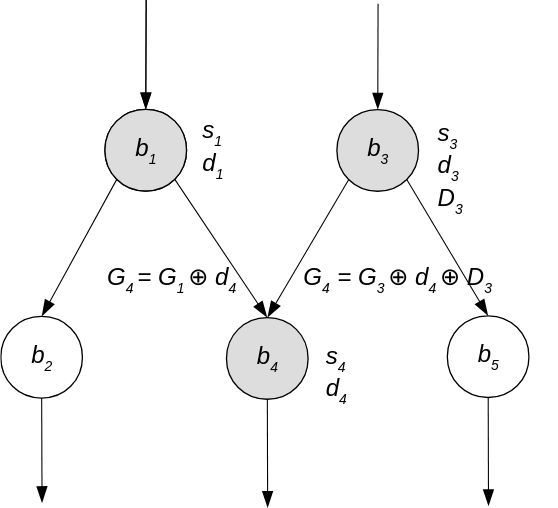
\includegraphics[width=0.6\textwidth]{diagrams/cfcss/adjuster.png}
    \caption{\acrshort{cfcss} with fan-in block \cite{coast:cfcss}}
\end{figure}

We need to introduce another constant called signature adjuster ({$D_n$}) calculated for each predecessor of a fan-in node, and apply it while updating the runtime signature. The adjuster is generated by XORing the signature of the current node ({$s_n$}) with the signature of the successor ({$s_{n+1}$}). This gives us the actual equation (\ref{eq:runtime_sig_with_adj}) for updating runtime signature.

\begin{equation}
\label{eq:runtime_sig_with_adj}
G_n = G_{n-1} \oplus d_n \oplus D_n
\end{equation}

\subsubsection{Macro implementation}

The Rust macro generates static variables ({$G_n, D_n, s_n, d_n$}) during compile time and inserts additional code before and after the actual function code within the protected module (see figure \ref{fig:rust_cfcss_macro}). The instructions inserted after the function block are equivalent to the ones inserted before, with the exception of restoring \textit{last adjuster} from stack instead of updating and storing it.

\begin{figure}[!h]
\begin{lstlisting}[language=Rust]
RUNTIME_SIGNATURE ^= #dif_name;
if is_fan_in {
    RUNTIME_SIGNATURE ^= RUNTIME_ADJUSTER;
}
if #sig_name != RUNTIME_SIGNATURE {
    return_to_checkpoint(ERROR_MSG);
}
if func_has_adjuster {
    RUNTIME_ADJUSTER = #adj_name;
}
\end{lstlisting}
\caption{Rust - \acrshort{cfcss} instructions inserted before function block}
\label{fig:rust_cfcss_macro}
\end{figure}

This macro can be applied as shown in figure \ref{fig:rust_cfcss_macro_example} by specifying a module as \textit{\#[cfcss\_root]}. An entry function is designated with a special macro \textit{\#[entry]}, this macro embeds additional instruction that reset the runtime signature and adjuster of the module, allowing for repeated call of the entry point. An entry function can only be a function that is not called from within another function in the protected module (module being a collection of functions designated as seen in Fig. \ref{fig:rust_cfcss_macro_example} line 2).

\begin{figure}[!h]
\begin{lstlisting}[language=Rust]
#[cfcss_root]
pub mod protected_block {
    fn function_0();
    fn function_1();
    #[entry]
    pub fn entry_function() {
        function_0();
        function_1();
    }
}
\end{lstlisting}
\caption{Rust - Using the \acrshort{cfcss} macro}
\label{fig:rust_cfcss_macro_example}
\end{figure}

\subsubsection{Overhead}

Embedding new instruction during compile time will understandably have performance impact on the execution of the program. Each function will incur a execution overhead, as multiple operations and checks must be carried out before the actual function body executes. Approximately 50 additional assembly instructions are inserted before the function block and 50 more after the function block, without using any compiler optimizations.

However, due to the nature of the implementation, the developer is in full control of just how much overhead is incurred. Since the number of additional instructions is constant per function definition, we can either split our protected module into fewer function to have less overhead, but at the cost of lower fault-tolerance. Or we can fragment our code into as many function blocks as possible, and thereby increasing the number of control flow checks performed.

\subsubsection{Considerations}

Since our implementation of \acrshort{cfcss} utilizes a purely code based approach it naturally comes with several limitations. Unlike the traditional approach, which implements \acrshort{cfcss} at \acrshort{ir} level by extending the LLVM pipeline we do not have access to the underlying instructions, which limits the possible density of the control flow checks. An \acrshort{ir} approach is able to precisely insert instructions after every branch and jump operations, and also has more granular control over the actual instructions being inserted. This means our implementation is more prone to control flow errors. Although not within the extent of this thesis, further improvements could be made by directly extending Rust's LLVM pipeline and integrating a \acrshort{cfcss} method at \acrshort{ir} level.

Additionally, \acrshort{cfcss} is incompatible with the aforementioned checkpoint and restart system. As explained in section \ref{sec:checkpoint_considerations}, our checkpoint and restart system does not restore context of static variables, which \acrshort{cfcss} relies on for proper functioning. 
% As such, checkpoints cannot be used within a \acrshort{cfcss} protected module, since if a checkpoint restart were to happen, the runtime signature and adjuster would not be reset to their proper pre-checkpoint values.